%%%%%%%%%%%%%%%%%%%%%%%%%%%%%%%%%%%%%%%%%
% Beamer Presentation
% LaTeX Template
% Version 1.0 (10/11/12)
%
% This template has been downloaded from:
% http://www.LaTeXTemplates.com
%
% License:
% CC BY-NC-SA 3.0 (http://creativecommons.org/licenses/by-nc-sa/3.0/)
%
%%%%%%%%%%%%%%%%%%%%%%%%%%%%%%%%%%%%%%%%%

%----------------------------------------------------------------------------------------
%	PACKAGES AND THEMES
%----------------------------------------------------------------------------------------

\documentclass{beamer}

\mode<presentation> {

% The Beamer class comes with a number of default slide themes
% which change the colors and layouts of slides. Below this is a list
% of all the themes, uncomment each in turn to see what they look like.

%\usetheme{default}
%\usetheme{AnnArbor}
%\usetheme{Antibes}
%\usetheme{Bergen}
%\usetheme{Berkeley}
%\usetheme{Berlin}
%\usetheme{Boadilla}
%\usetheme{CambridgeUS}
%\usetheme{Copenhagen}
%\usetheme{Darmstadt}
%\usetheme{Dresden}
%\usetheme{Frankfurt}
%\usetheme{Goettingen}
%\usetheme{Hannover}
%\usetheme{Ilmenau}
%\usetheme{JuanLesPins}
%\usetheme{Luebeck}
\usetheme{Madrid}
%\usetheme{Malmoe}
%\usetheme{Marburg}
%\usetheme{Montpellier}
%\usetheme{PaloAlto}
%\usetheme{Pittsburgh}
%\usetheme{Rochester}
%\usetheme{Singapore}
%\usetheme{Szeged}
%\usetheme{Warsaw}

% As well as themes, the Beamer class has a number of color themes
% for any slide theme. Uncomment each of these in turn to see how it
% changes the colors of your current slide theme.

%\usecolortheme{albatross}
%\usecolortheme{beaver}
%\usecolortheme{beetle}
%\usecolortheme{crane}
%\usecolortheme{dolphin}
%\usecolortheme{dove}
%\usecolortheme{fly}
%\usecolortheme{lily}
%\usecolortheme{orchid}
%\usecolortheme{rose}
%\usecolortheme{seagull}
%\usecolortheme{seahorse}
%\usecolortheme{whale}
%\usecolortheme{wolverine}

%\setbeamertemplate{footline} % To remove the footer line in all slides uncomment this line
%\setbeamertemplate{footline}[page number] % To replace the footer line in all slides with a simple slide count uncomment this line

%\setbeamertemplate{navigation symbols}{} % To remove the navigation symbols from the bottom of all slides uncomment this line
}

\usepackage{graphicx} % Allows including images
\usepackage{booktabs} % Allows the use of \toprule, \midrule and \bottomrule in tables
\usepackage[brazilian]{babel}
\usepackage[utf8]{inputenc}
\usepackage[T1]{fontenc}



%----------------------------------------------------------------------------------------
%	TITLE PAGE
%----------------------------------------------------------------------------------------

\title[MQTT]{MQTT} % The short title appears at the bottom of every slide, the full title is only on the title page

\author{Gabriel R. Caldas de Aquino} % Your name
\institute[UFRJ] % Your institution as it will appear on the bottom of every slide, may be shorthand to save space
{
Universidade Federal do Rio de Janeiro \\ % Your institution for the title page
\medskip
\textit{gabriel@labnet.nce.ufrj.br} % Your email address
}
\date{\today} % Date, can be changed to a custom date

\begin{document}

\begin{frame}
\titlepage % Print the title page as the first slide
\end{frame}

%\begin{frame}
%\frametitle{\'{I}ndice} % Table of contents slide, comment this block out to remove it
%\tableofcontents % Throughout your presentation, if you choose to use \section{} and \subsection{} commands, these will automatically be printed on this slide as an overview of your presentation
%\end{frame}

%----------------------------------------------------------------------------------------
%	PRESENTATION SLIDES
%----------------------------------------------------------------------------------------

%------------------------------------------------
\section{Introdu\c{c}\~ao} % Sections can be created in order to organize your presentation into discrete blocks, all sections and subsections are automatically printed in the table of contents as an overview of the talk


%------------------------------------------------
\begin{frame}
\frametitle{Introdu\c{c}\~ao}
\begin{itemize}
\item Criado em 1999 para conectar oleodutos por conex\~{a}o via sat\'{e}lite;
\item Caracter\'{i}sticas:
	\begin{itemize}
	\item Open Source
    \item Simples e f\'{a}cil de implementar
    \item Leve e consome pouca banda
    \item Prov\^{e} QoS
    \item Agn\'{o}stico de dados: depende de como o payload é estruturado
	\end{itemize}

\item Interessante para dispositivos de recursos limitados;
	\begin{itemize}
	\item Comunica\c{c}\~{a}o M2M na IoT;
	\end{itemize}

\item Versão atual 3.1.1;


\end{itemize}
\end{frame}

%------------------------------------------------

\begin{frame}
\frametitle{Introdu\c{c}\~ao}

\begin{itemize}
\item Protocolo de transporte de mensagens cliente servidor do tipo publish/subscribe:
	\begin{itemize}
	\item Existem t\'{o}picos;
    \item Clientes publicam em t\'{o}picos;
    \item Clientes assinam determinados t\'{o}picos.
	\end{itemize}

\end{itemize}

\begin{figure}
\centering
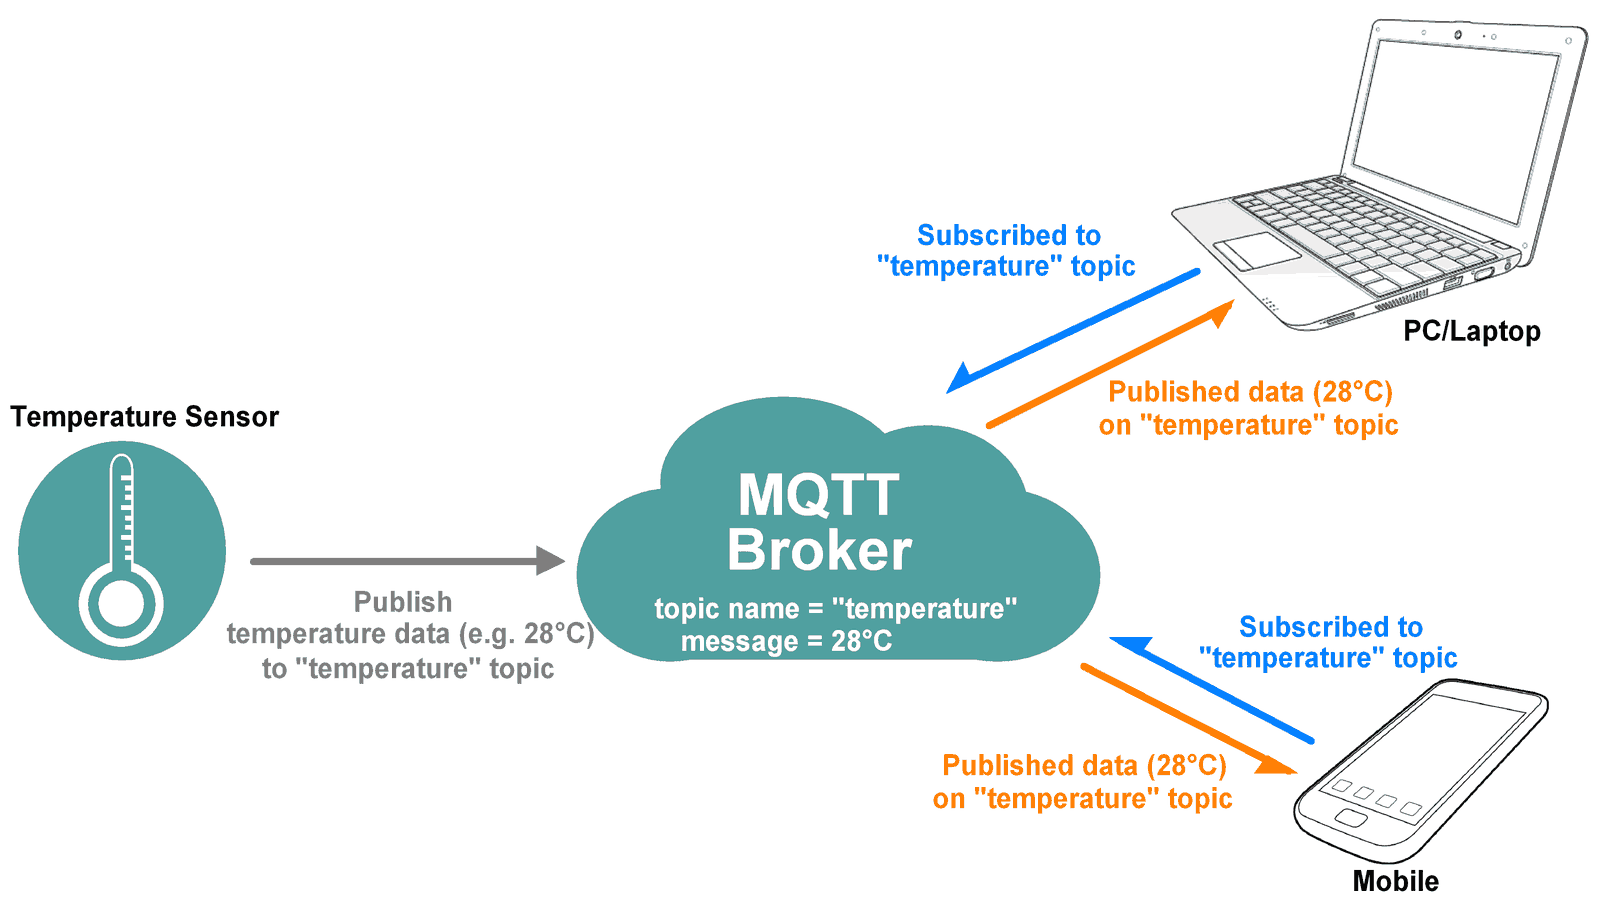
\includegraphics[scale=0.2]{MQTT1}
\end{figure}

\end{frame}
%------------------------------------------------

\begin{frame}
\frametitle{Din\'{a}mica de Pub/Sub}




	\begin{itemize}
	\item Tanto publisher quanto subscriber se conectam a um broker
    \item Clientes escrevem em um t\'{o}pico
    \item Broker recebe as mensagens e as distribui
    \item Se um t\'{o}pico receber uma nova mensagem, o broker envia aos clientes
    
	\end{itemize}
    
%\item REST-ful Api Web:

%	\begin{itemize}
%	\item Clientes se comunicam diretamente com um servidor tradicional (geralmente WEB)
%    \item Clientes se usam API WEB para enviar os dados
%    \item Os dados ficam guardados no servidor
%    \item Cliente requisitam através de API WEB
%    \item Geralmente a consulta é feita através de REST-ful APIs
%	\end{itemize}


\end{frame}

%------------------------------------------------
\begin{frame}
\frametitle{O broker}

\begin{block}{MQTT broker}   
    O broker é o responsável por receber mensagens, filtrar, decidir quem está interessado e enviar a todos os clientes inscritos.
\end{block}

\begin{itemize}

\item Parte principal do Publish/Subscribe
\item Mant\'{e}m a sessão dos clientes (assinaturas e mensagens perdidas)
\item Autentica\c{c}\~ao e autoriza\c{c}\~ao de clientes
\item \'{E} geralmente extens\'{i}vel: c\'{o}digo aberto

\begin{block}{\'{E} importante que:}      
	O Broker seja \emph{escalável}, \emph{integr\'{a}vel}, \emph{monitor\'{a}vel} e \emph{tolerante a falhas}.
\end{block}    

\end{itemize}
\end{frame}

%------------------------------------------------


\begin{frame}
\frametitle{Exemplos de brokers}
\begin{itemize}

\item Eclipse Mosquitto: https://mosquitto.org/
	\begin{itemize}
	\item Open source (EPL/EDL licensed) 
	\item Implementa o protocolo MQTT ver. 3.1 e 3.1.1. 
	\end{itemize}
    
\item Hivemq: https://www.hivemq.com/
	\begin{itemize}
	\item Compat\'{i}vel com MQTT 3.1 e 3.1.1 
	\item Solu\c{c}\~ao mais completa
	\end{itemize}
    
\item Lista: https://github.com/mqtt/mqtt.github.io/wiki/brokers

\end{itemize}
\end{frame}


%------------------------------------------------


\begin{frame}
\frametitle{Os clientes}

\begin{block}{Cliente MQTT}
Qualquer dispositivo que execute as bibliotecas do MQTT e est\'{a} conectado a um broker MQTT em qualquer tipo de rede.
\end{block}
\begin{itemize}
\item Basicamente qualquer dispositivo conectado a um broker:

\item Dispositivo pequeno e com recursos limitados conectado por uma rede sem fio. 
\item Computador t\'{i}pico executando um cliente MQTT.

\end{itemize}

\end{frame}

%------------------------------------------------

\begin{frame}
\frametitle{MQTT e a Pilha TCP/IP}
\begin{itemize}
\item MQTT funciona sobre a pilha TCP/IP
\item TCP/IP porta 1883
\end{itemize}
\begin{figure}
\centering
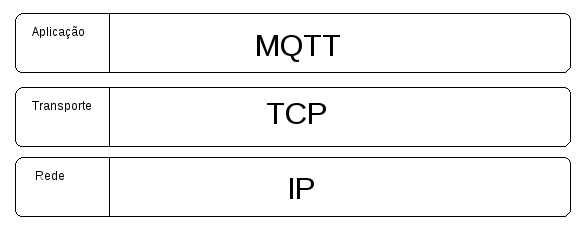
\includegraphics[scale=0.5]{MQTT2}
\end{figure}
\end{frame}

%------------------------------------------------

\begin{frame}
\frametitle{Formato do pacote de controle MQTT}
\begin{itemize}
\item O pacote consiste em at\'{e} tr\^{e}s partes (na seguinte ordem):
\end{itemize}
\begin{figure}
\centering
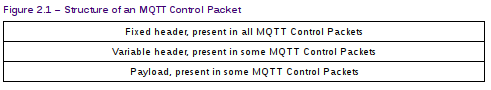
\includegraphics[scale=0.7]{MQTT-Formato-PKT}
\end{figure}
\end{frame}

%------------------------------------------------

\begin{frame}
\frametitle{Header Fixo MQTT}
\begin{itemize}
\item O Header Fixo do pacote MQTT \'{e} dividido em tr\^{e}s peda\c{c}os:
\end{itemize}
\begin{figure}
\centering
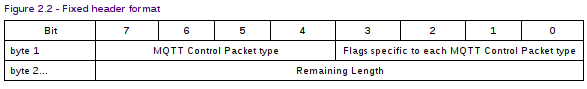
\includegraphics[scale=0.6]{MQTT-FixedHeader-Format}
\end{figure}
\end{frame}

%------------------------------------------------

\begin{frame}
\frametitle{Header Fixo MQTT - Tipos de pacote de controle}
\begin{itemize}
\item 4-bit unsigned values (byte 4 ao 7):
\end{itemize}
\begin{figure}
\centering
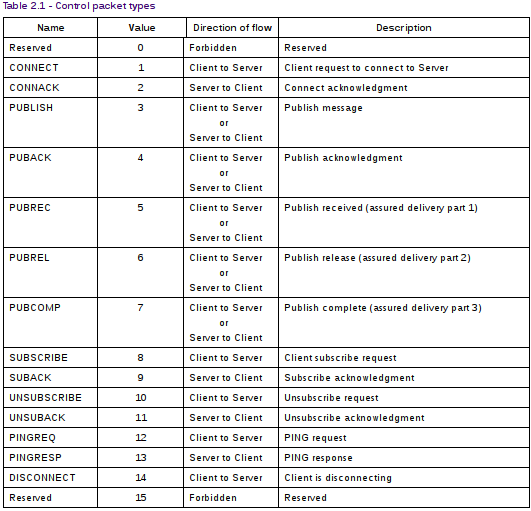
\includegraphics[scale=0.4]{MQTT-TypesOfControlPackets}
\end{figure}
\end{frame}

%------------------------------------------------

\begin{frame}
\frametitle{Header Fixo MQTT - Flags}
\begin{itemize}
\item 4-bit unsigned values (byte 0 ao 3):
\end{itemize}
\begin{figure}
\centering
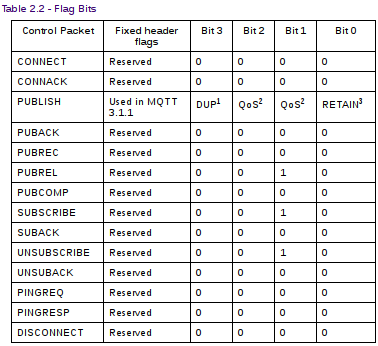
\includegraphics[scale=0.5]{MQTT-FixedHeader-Flags}
\end{figure}
\end{frame}

%------------------------------------------------

\begin{frame}
\frametitle{Header variável MQTT}

%\begin{figure}
%\centering
%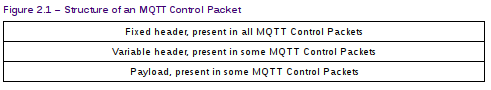
\includegraphics[scale=0.3]{MQTT-Formato-PKT}
%\end{figure}

\begin{figure}
\centering
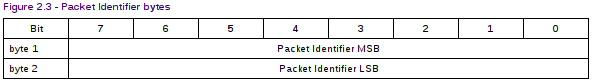
\includegraphics[scale=0.3]{MQTT-PacketIdentifier}
\end{figure}

\begin{figure}
\centering
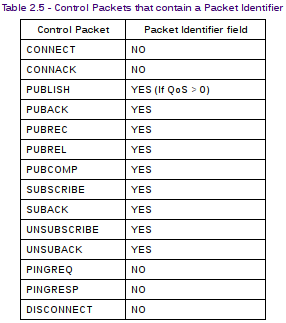
\includegraphics[scale=0.5]{MQTT-ControlPacketsWithIdentifier}
\end{figure}


\end{frame}

%------------------------------------------------

\begin{frame}
\frametitle{Payload MQTT}

\begin{figure}
\centering
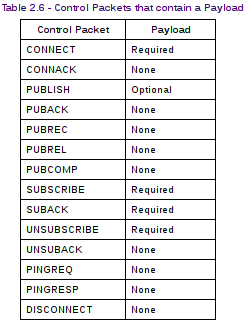
\includegraphics[scale=0.5]{MQTT-ControlPacketsWithPayload}
\end{figure}


\end{frame}

%------------------------------------------------

\begin{frame}
\frametitle{Estabelecendo uma conexão MQTT}

\begin{itemize}
\item A conexão MQTT é sempre entre um cliente e o broker
\item Não há conexão entre clientes
\end{itemize}

\begin{figure}
\centering

\includegraphics[scale=0.5]{MQTT-ConnectionStablishment}
\end{figure}

\begin{itemize}
\item Uma vez que a conexão é estabelecida o Broker a mantém aberta
\item A conexão só fecha com uma mensagem de disconnect ou quando a conexão é perdida
\end{itemize}


\end{frame}

%------------------------------------------------

\begin{frame}
\frametitle{Formato dos pacotes Connect e Connackdo MQTT}

\begin{figure}
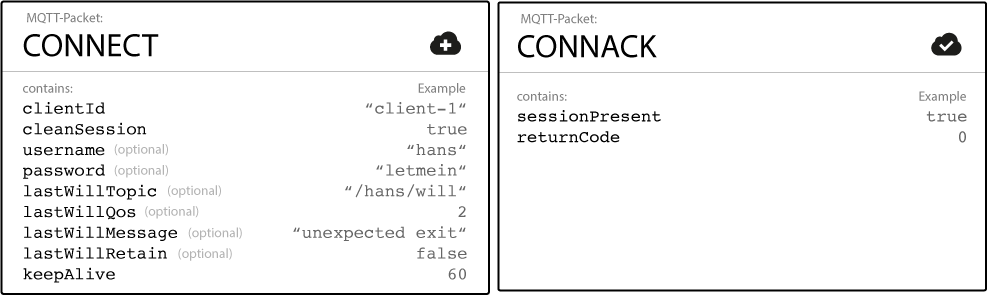
\includegraphics[scale=0.35]{MQTT-Connect+Connack}
%\raggedleft
\end{figure}

%\begin{figure}
%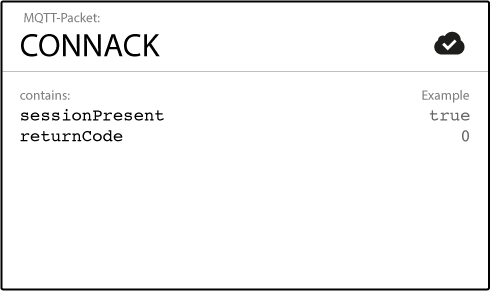
\includegraphics[scale=0.3]{MQTT-ConnackMsg}
%\raggedright
%\end{figure}

\begin{table}[]
\centering
%\caption{My caption}
%\label{my-label}
\scalebox{0.4}{
\begin{tabular}{lll}
 Return Code&  Return Code Response& \\
 0&  Connection Accepted& \\
 1&  Connection Refused, unacceptable protocol version& \\
 2&  Connection Refused, identifier rejected& \\
 3&  Connection Refused, Server unavailable& \\
 4&  Connection Refused, bad user name or password& \\
 5&  Connection Refused, not authorized& 

\end{tabular}
}
\end{table}


\end{frame}
%------------------------------------------------

\begin{frame}
\frametitle{Publicando no MQTT}

\begin{itemize}
\item Após conectado, o cliente pode publicar no Broker
\item MQTT filtra e passa as mensagens por tópicos

\begin{itemize}
\item Cada mensagem \emph{publish} tem que conter um tópico
\item Este tópico é usado pelo broker para encaminhar as mensagens aos clientes interessados.
\end{itemize}

\item Cada mensagem contêm os bytes dos dados para transmitir
\end{itemize}


\begin{block}{}   
    O MQTT não possui conhecimento acerca dos dados. Ou seja, o uso depende totalmente do caso e de como a mensagem é estruturada. Cabe ao usuário como estruturar o envio dos dados: dados binários, dados textuais ou mesmo XML ou JSON completos.
\end{block}


\end{frame}
%------------------------------------------------

\begin{frame}
\frametitle{Publicando no MQTT}

\begin{block}{}
Quando um cliente publica, o broker lê a publicação, confirma de acordo com o QoS e, em seguida processa. O processamento é determinar os clientes inscritos e depois enviar aos clientes selecionados.
\end{block}

\begin{figure}
\centering
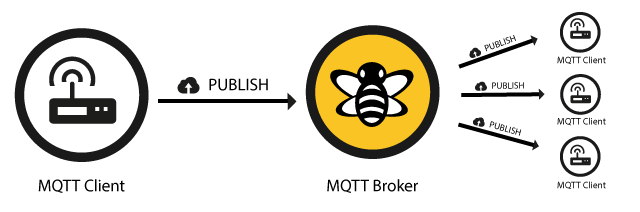
\includegraphics[scale=0.3]{MQTT-PublishFlow}
\end{figure}

\begin{itemize}
\item Quem publica a mensagem está preocupado apenas em entregar a mensagem ao broker.
\item Então, é responsabilidade do broker entregar a mensagem a todos os subscribers
\item O cliente que publicou não recebe nenhum feedback dos assinantes

\end{itemize}


\end{frame}

%------------------------------------------------

\begin{frame}
\frametitle{Estrutura do pacote \emph{publish}}
\begin{figure}
\centering
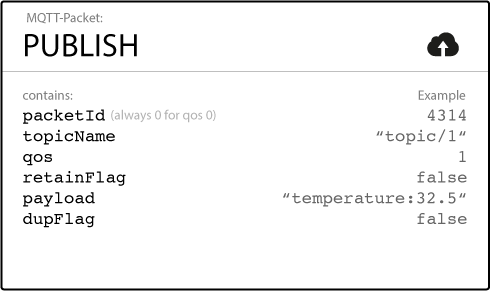
\includegraphics[scale=0.3]{MQTT-PublishPacket}
\end{figure}
\begin{itemize}
\item \emph{Packet Identifier}: É relevante para o QoS
\item \emph{Topic Name}: Uma string estruturada hierarquicamente. Ex: casa/sala/luz
\item \emph{QoS}: Determina a garantia de entrega ao cliente ou broker
\item \emph{Retain-Flag}: Determina se a mensagem será salva pelo broker. Novos clientes recebem a mensagem após a inscrição. 
\item \emph{Payload}: É o conteúdo da mensagem
\item \emph{DUP flag}: indica que esta mensagem é duplicada e é reenviada porque a outra extremidade não confirmou a mensagem original
\end{itemize}


\end{frame}



%------------------------------------------------

\begin{frame}
\frametitle{Assinando e cancelando a assinatura}

\begin{figure}
\centering
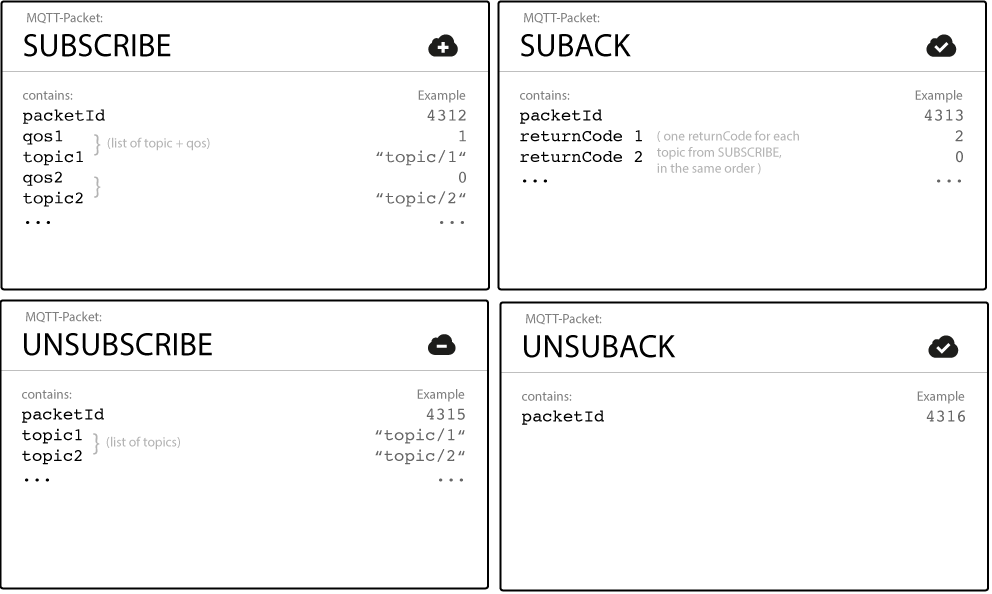
\includegraphics[scale=0.25]{MQTT-SUBUNSUB}
\end{figure}

\begin{figure}
\centering
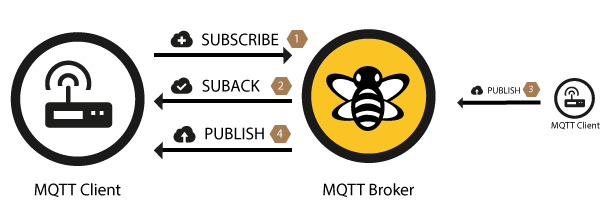
\includegraphics[scale=0.3]{MQTT-SubPubFlow}
\end{figure}

\end{frame}

%------------------------------------------------

\begin{frame}
\frametitle{Tópicos}
\begin{itemize}
\item Estrutura hierárquica (Lembra pastas de um S.O.) em forma de string UTF-8
\item usa a barra (/) como um delimitador
\item Tópicos são case-sensitive e devem ao menos conter um caracter válido
\item Exemplos:
\begin{itemize}
\item house/room/main-light
\item house/room/side-light
\item house/garage/main-light
\item house/garage/alarm
\end{itemize}
\end{itemize}

\begin{block}{}
Diferentes tópicos podem ser assinados usando  \emph{wildcards}
\end{block}

\end{frame}


%------------------------------------------------

\begin{frame}
\frametitle{Usando \emph{wildcards}}

\begin{itemize}

\item Existem dois tipos:

\begin{itemize}
\item \#: \emph{wildcard} de vários níveis
\item +: \emph{wildcard} de um único nivel
\end{itemize}

\item Exemplo: house/+/main-light

\begin{itemize}
\item (cobre) house/room1/main-light
\item (cobre) house/room2/main-light
\item (não cobre) house/room1/side-light
\end{itemize}

\item Exemplo 2: house/\#
\begin{itemize}
\item (cobre) house/room1/main-light
\item (cobre) house/room1/alarm
\item (cobre) house/garage/main-light
\item (cobre) house/main-door
\end{itemize}
\end{itemize}

\end{frame}
%------------------------------------------------

\begin{frame}
\frametitle{Um pouco além: QoS}

3 níveis de QoS no MQTT:
\begin{itemize}
\item 3 níveis de QoS no MQTT:

\begin{itemize}
\item No máximo uma vez (0) (Best-Effort): Uma mensagem não será confirmada pelo destinatário nem será armazenada e devolvida pelo remetente
\item Pelo menos uma vez (1): É garantido que uma mensagem será entregue pelo menos uma vez ao destinatário. Mas a mensagem também pode ser entregue mais de uma vez.

\item Exatamente uma vez (2): Garante que cada mensagem seja recebida apenas uma vez pela contraparte. É a qualidade mais segura e também a mais lenta do nível de serviço.
\end{itemize}
\end{itemize}

\begin{block}{Importante:}
É importante dizer que quanto maior o nível de QoS, maior é a troca de mensagens e o consquente overhead na rede.
\end{block}
\end{frame}

%------------------------------------------------






\begin{frame}
\frametitle{References}
\begin{itemize}
\item http://docs.oasis-open.org/mqtt/mqtt/v3.1.1/mqtt-v3.1.1.html
\item https://www.hivemq.com/blog/mqtt-essentials/
\item http://www.steves-internet-guide.com/understanding-mqtt-topics/
\end{itemize}
\end{frame}

%------------------------------------------------

\begin{frame}
\Huge{\centerline{Obrigado}}
\end{frame}

%----------------------------------------------------------------------------------------

\end{document}